\section{Ejercicio 5 - Crear una jerarquía}  

1. En el Diseñador de dimensiones para la dimensión DimDate, arrastre el atributo Calendar Year del panel
Atributos al panel Jerarquías

	\begin{center}
	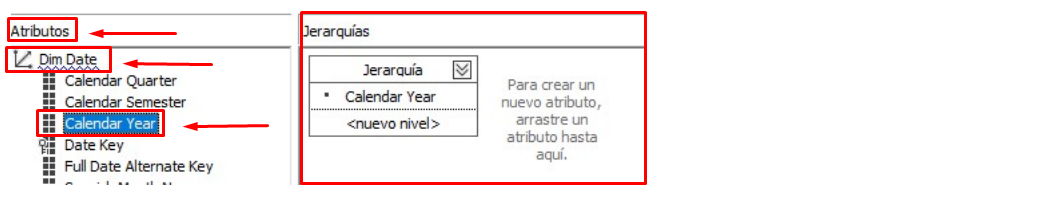
\includegraphics[width=\columnwidth]{images/task5/img1}
	\end{center}	

2. Arrastre el atributo Calendar Semester del panel Atributos a la celda <nuevo nivel> del panel Jerarquías, debajo
del nivel Calendar Year

3.Arrastre el atributo Calendar Quarter del panel Atributos a la celda <nuevo nivel> del panel Jerarquías, debajo
del nivel Calendar Semester.

4. Arrastre el atributo Spanish Month Name del panel Atributos a la celda <nuevo nivel> del panel Jerarquías, debajo del nivel Calendar Quarter.

5. Arrastre el atributo Date Key del panel Atributos a la celda <nuevo nivel> del panel Jerarquías, debajo del nivel
Spanish Month Name.

	\begin{center}
	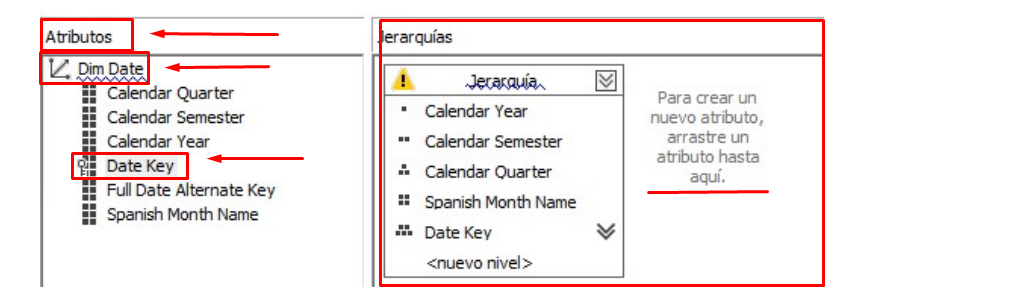
\includegraphics[width=\columnwidth]{images/task5/img2}
	\end{center}	

6. En el panel Jerarquías, haga clic derecho en la barra de título de la jerarquía Jerarquía, seleccione Cambiar nombre
y escriba Calendar Date.

7. En la jerarquía Calendar Date, cambie el nombre del nivel Spanish Month Name a Calendar Month y el del nivel
Date Key a Date.

	\begin{center}
	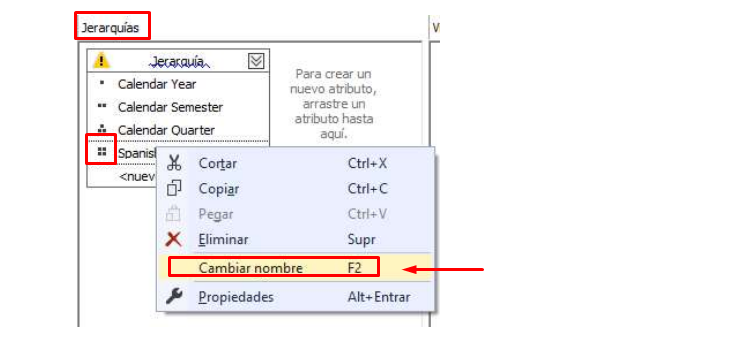
\includegraphics[width=\columnwidth]{images/task5/img3}
	\end{center}	

	\begin{center}
	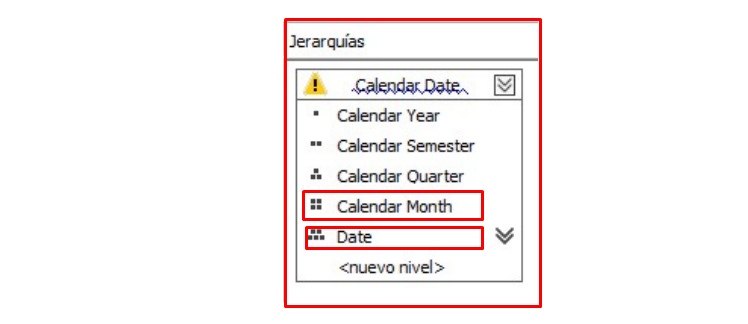
\includegraphics[width=\columnwidth]{images/task5/img4}
	\end{center}	

8. Elimine el atributo FullDateAlternateKey del panel Atributos, ya que no lo va a usar.

	\begin{center}
	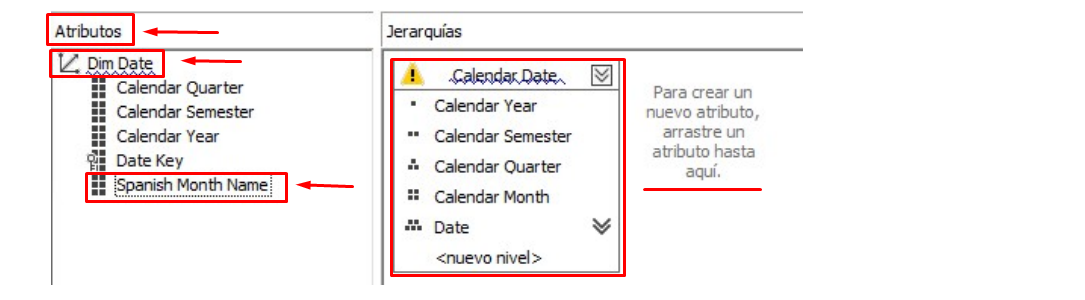
\includegraphics[width=\columnwidth]{images/task5/img5}
	\end{center}	

9. Verificar las relaciones del atributo DateKey en la pestaña Realaciones de atributo

	\begin{center}
	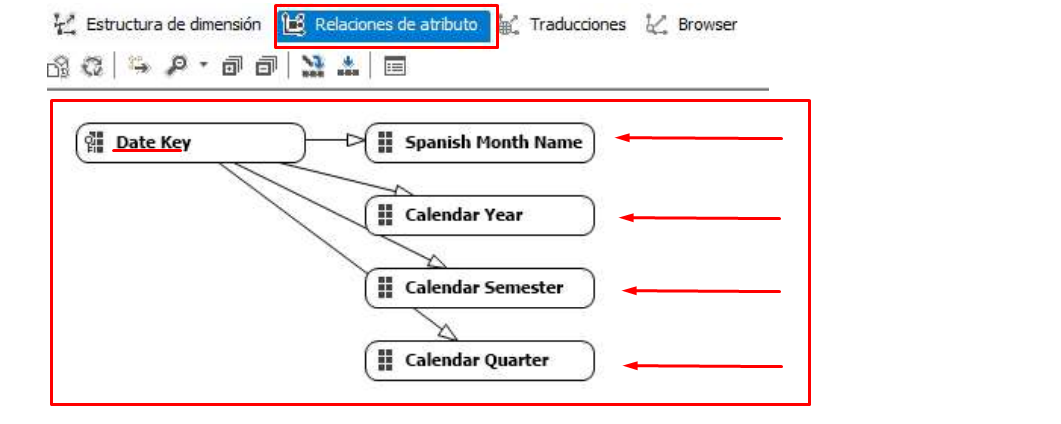
\includegraphics[width=\columnwidth]{images/task5/img6}
	\end{center}	

10. En el menú Archivo del proyecto, haga clic en Guardar todo

    